\documentclass[aspectratio=169]{../latex_main/tntbeamer}  % you can pass all options of the beamer class, e.g., 'handout' or 'aspectratio=43'
\usepackage{dsfont}
\usepackage{bm}
\usepackage[english]{babel}
\usepackage[T1]{fontenc}
%\usepackage[utf8]{inputenc}
\usepackage{graphicx}
\graphicspath{ {./figures/} }
\usepackage{algorithm}
\usepackage[ruled,vlined,algo2e,linesnumbered]{algorithm2e}
\usepackage{hyperref}
\usepackage{booktabs}
\usepackage{mathtools}

\usepackage{amsmath,amssymb}

\DeclareMathOperator*{\argmax}{arg\,max}
\DeclareMathOperator*{\argmin}{arg\,min}

\usepackage{amsbsy}
\newcommand{\vect}[1]{\bm{#1}}
%\newcommand{\vect}[1]{\boldsymbol{#1}}

\usepackage{pgfplots}
\pgfplotsset{compat=1.16}
\usepackage{tikz}
\usetikzlibrary{trees} 
\usetikzlibrary{shapes.geometric}
\usetikzlibrary{positioning,shapes,shadows,arrows,calc,mindmap}
\usetikzlibrary{positioning,fadings,through}
\usetikzlibrary{decorations.pathreplacing}
\usetikzlibrary{intersections}
\pgfdeclarelayer{background}
\pgfdeclarelayer{foreground}
\pgfsetlayers{background,main,foreground}
\tikzstyle{activity}=[rectangle, draw=black, rounded corners, text centered, text width=8em]
\tikzstyle{data}=[rectangle, draw=black, text centered, text width=8em]
\tikzstyle{myarrow}=[->, thick, draw=black]

% Define the layers to draw the diagram
\pgfdeclarelayer{background}
\pgfdeclarelayer{foreground}
\pgfsetlayers{background,main,foreground}

% Requires XeLaTeX or LuaLaTeX
%\usepackage{unicode-math}

\usepackage{fontspec}
%\setsansfont{Arial}
\setsansfont{RotisSansSerifStd}[ 
Path=../latex_main/fonts/,
Extension = .otf,
UprightFont = *-Regular,  % or *-Light
BoldFont = *-ExtraBold,  % or *-Bold
ItalicFont = *-Italic
]
\setmonofont{Cascadia Mono}[
Scale=0.8
]

% scale factor adapted; mathrm font added (Benjamin Spitschan @TNT, 2021-06-01)
%\setmathfont[Scale=1.05]{Libertinus Math}
%\setmathrm[Scale=1.05]{Libertinus Math}

% other available math fonts are (not exhaustive)
% Latin Modern Math
% XITS Math
% Libertinus Math
% Asana Math
% Fira Math
% TeX Gyre Pagella Math
% TeX Gyre Bonum Math
% TeX Gyre Schola Math
% TeX Gyre Termes Math

% Literature References
\newcommand{\lit}[2]{\href{#2}{\footnotesize\color{black!60}[#1]}}

%%% Beamer Customization
%----------------------------------------------------------------------
% (Don't) Show sections in frame header. Options: 'sections', 'sections light', empty
\setbeamertemplate{headline}{empty}

% Add header logo for normal frames
\setheaderimage{
	% 
\includegraphics[height=\logoheight]{figures/TNT_darkv4.pdf}
	
\includegraphics[height=\logoheight]{../latex_main/figures/luh_logo_rgb_0_80_155.pdf}
	% 
\includegraphics[height=\logoheight]{figures/logo_tntluh.pdf}
}

% Header logo for title page
\settitleheaderimage{
	% 
\includegraphics[height=\logoheight]{figures/TNT_darkv4.pdf}
	
\includegraphics[height=\logoheight]{../latex_main/figures/luh_logo_rgb_0_80_155.pdf}
	% 
\includegraphics[height=\logoheight]{figures/logo_tntluh.pdf}
}

% Title page: tntdefault 
\setbeamertemplate{title page}[tntdefault]  % or luhstyle
% Add optional title image here
%\addtitlepageimagedefault{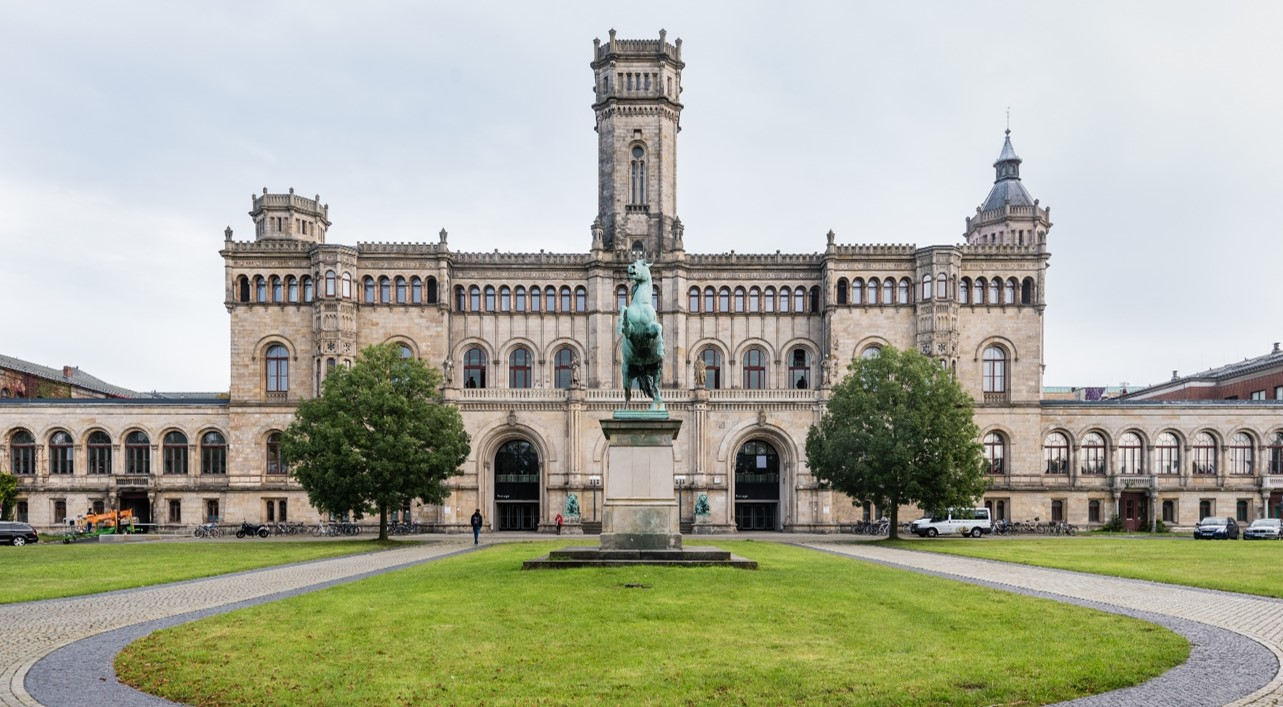
\includegraphics[width=0.65\textwidth]{figures/luh_default_presentation_title_image.jpg}}

% Title page: luhstyle
% \setbeamertemplate{title page}[luhstyle]
% % Add optional title image here
% \addtitlepageimage{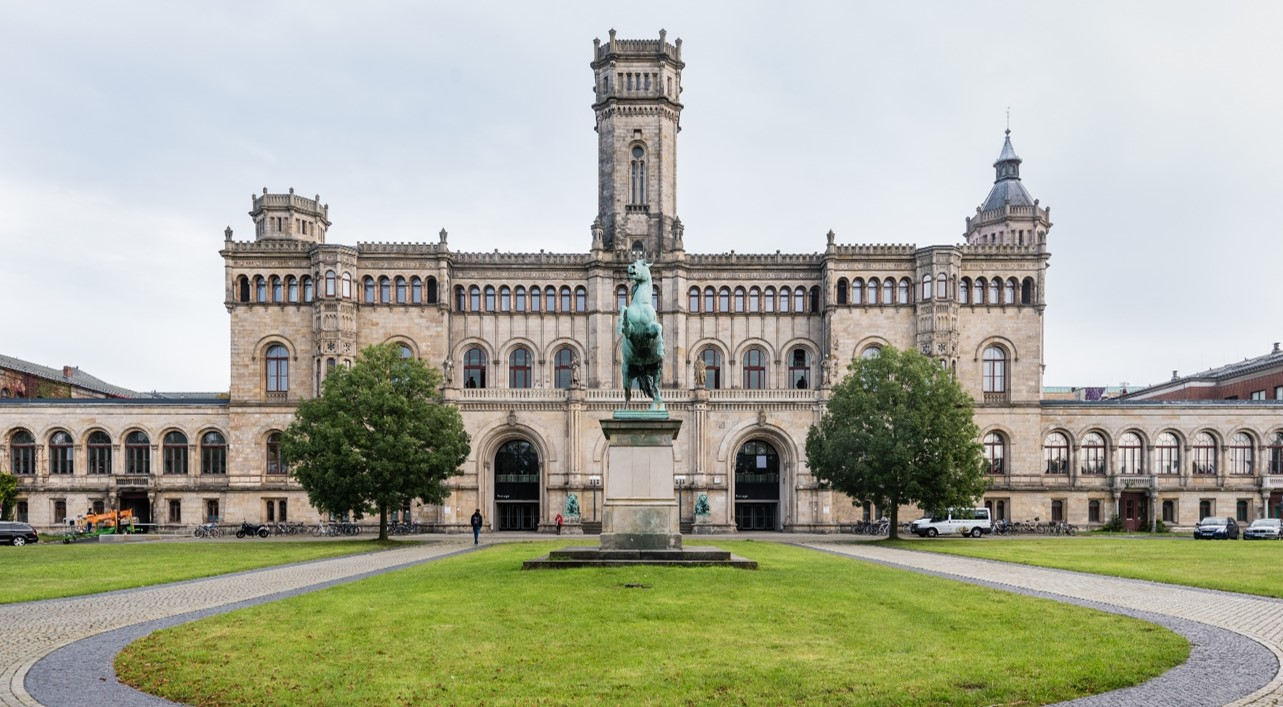
\includegraphics[width=0.75\textwidth]{figures/luh_default_presentation_title_image.jpg}}

\author[Abedjan \& Lindauer]{Ziawasch Abedjan \& Marius Lindauer\\[1em]
	
\includegraphics[height=\logoheight]{../latex_main/figures/luh_logo_rgb_0_80_155.pdf}\qquad
	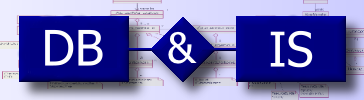
\includegraphics[height=\logoheight]{../latex_main/figures/DBIS_Kurzlogo.png}\qquad

\includegraphics[height=\logoheight]{../latex_main/figures/TNT_darkv4}\qquad

\includegraphics[height=\logoheight]{../latex_main/figures/L3S.jpg}	}
\date{Summer Term 2022; \hspace{0.5em} {
\includegraphics[height=1.5em]{../latex_main/figures/Cc-by-nc-sa_icon.svg.png}}; based on \href{https://ds100.org/fa21/}{[DS100]}
}


%%% Custom Packages
%----------------------------------------------------------------------
% Create dummy content
\usepackage{blindtext}

% Adds a frame with the current page layout. Just call \layout inside of a frame.
\usepackage{layout}


%%% Macros
%\renewcommand{\vec}[1]{\mathbf{#1}}
% \usepackage{bm}
%\let\vecb\bm

\title[Introduction]{DS: Regular Expressions}
\subtitle{Regular Expressions in Python (and Regex Groups)}

\graphicspath{ {./figure/} }
%\institute{}


\begin{document}
	
	\maketitle
	\begin{frame}{re.findall in Python}
	    In Python, re.findall(pattern, text) will return a list of all matches.
	    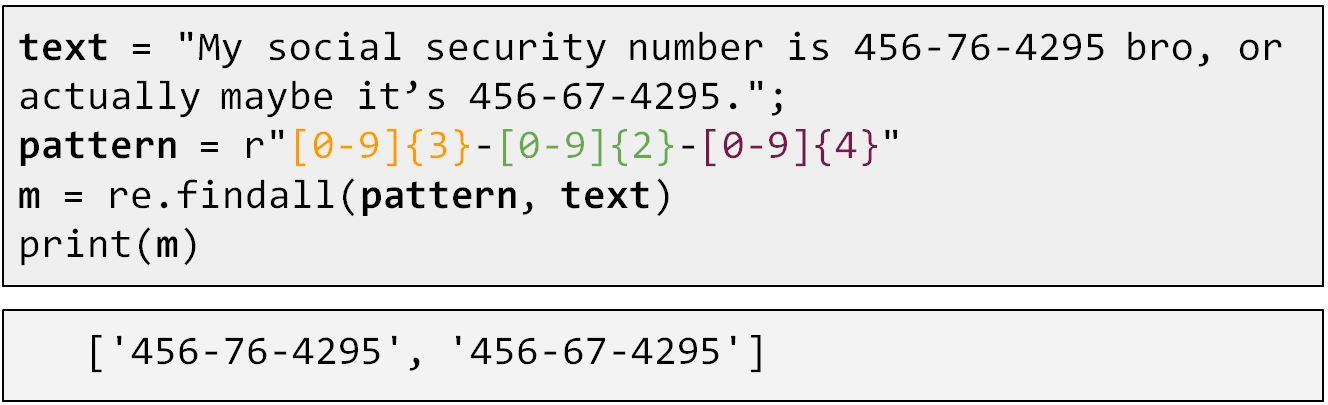
\includegraphics[scale=.35]{Bild19}
	\end{frame}
	
	
	\begin{frame}{re.sub in Python}
    	In Python, re.sub(pattern, repl, text) will return text with all instances of pattern replaced by repl.
	    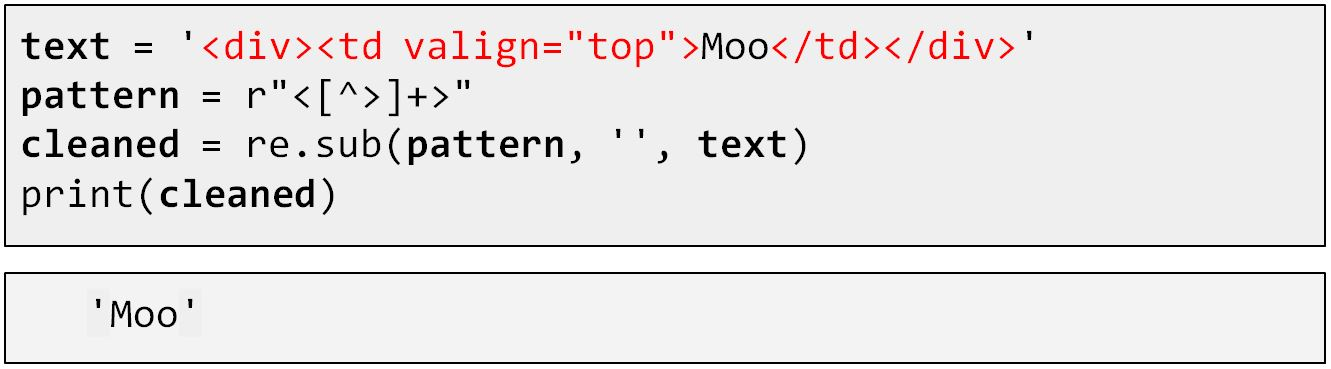
\includegraphics[scale=.35]{Bild20}
	\end{frame}
	
	
	\begin{frame}{Raw Strings in Python}
    	Note: When specifying a pattern, we strongly suggest using “raw strings”. 
    	\begin{itemize}
    	    \item A raw string is created using r“” or r‘’ instead of just “” or ‘’.
    	    \item The exact reason is a bit tedious.
    	    \begin{itemize}
    	        \item Rough idea: Regular expressions and Python strings both use \textbackslash as an escape character. 
    	        \item Using non-raw strings leads to uglier regular expressions.
    	    \end{itemize}
    	\end{itemize}
    	\begin{figure}
    	    \centering
    	    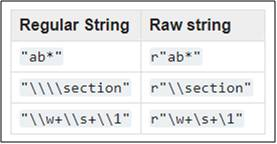
\includegraphics[scale=.5]{Bild21}
    	\end{figure}
	    
	    
	    
	    For more information see “The Backslash Plague” under \\
	    \url{https://docs.python.org/3/howto/regex.html}.
	\end{frame}
	
	
	\begin{frame}{Regular Expression Groups}
    	Earlier we used parentheses to specify the order of operations.\\
    	Parenthesis have another meaning:
    	\begin{itemize}
    	    \item Every set of parentheses specifies a so-called “group”. 
    	    \item Regular expression matchers (e.g. re.findall, \url{regex101.com}) will return matches organized by groups. In Python, returned as tuples.
    	\end{itemize}
    	\begin{figure}
    	    \centering
    	    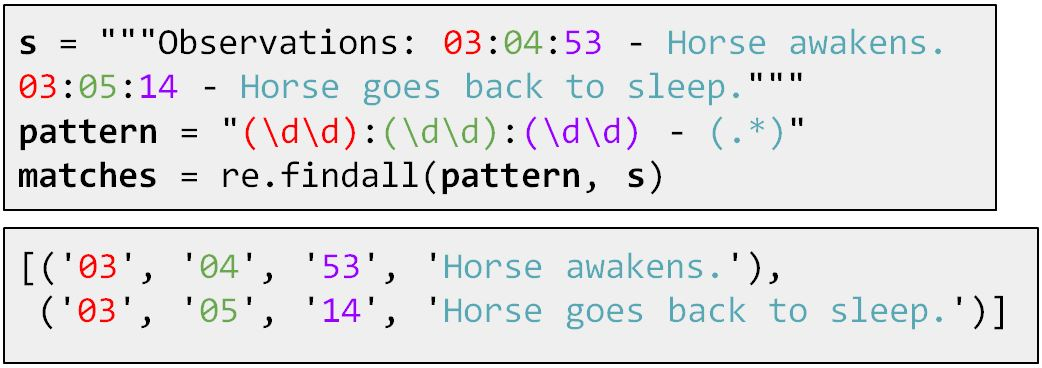
\includegraphics[scale=.35]{Bild22}
    	\end{figure}
	\end{frame}
	
	
	
	\begin{frame}{Regex Puzzle}
    	Fill in the regex below so that after code executes, day is “26”, month is “Jan”, and year is “2014”. 
    	\begin{itemize}
    	    \item See lec08-working-with-text.ipynb or \url{https://tinyurl.com/reg913s}.
    	\end{itemize}
    	\begin{figure}
    	    \centering
    	    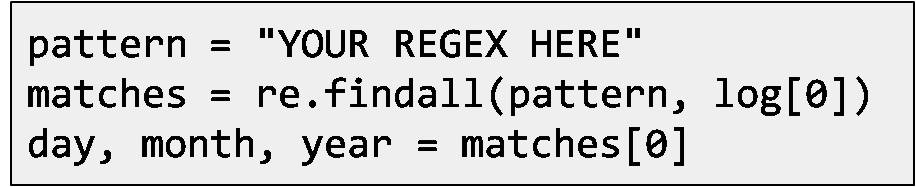
\includegraphics[scale=.6]{Bild23}
    	    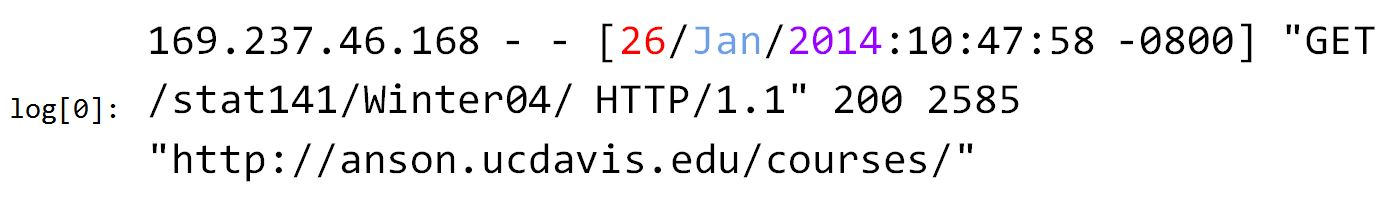
\includegraphics[scale=.4]{Bild27}
    	\end{figure}
	\end{frame}
	
	
	\begin{frame}{Regex Puzzle (One Possible Solution) }
    	Fill in the regex below so that after code executes, day is “26”, month is “Jan”, and year is “2014”. 
    	\begin{figure}
    	    \centering
    	    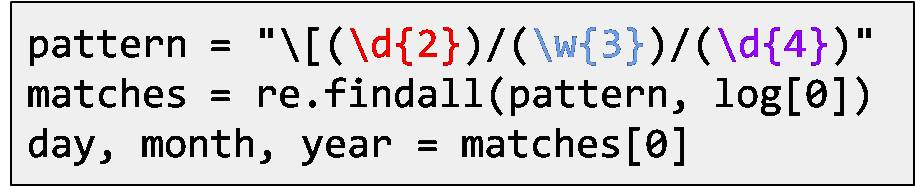
\includegraphics[scale=.6]{Bild24}
    	    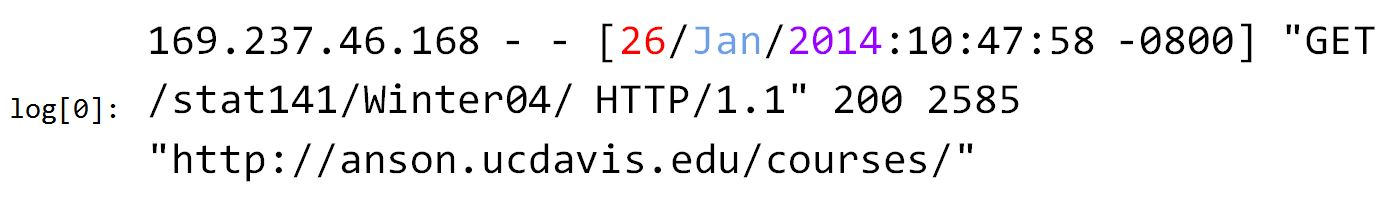
\includegraphics[scale=.4]{Bild27}
    	\end{figure}
	\end{frame}
	
	
	
	\begin{frame}{Extracting Date Information}
    	With a little more work, we can do something similar and extract day, month, year, hour, minutes, seconds, and time zone all in one regular expression.
    	\begin{itemize}
    	    \item Derivation is left as an exercise for you
    	\end{itemize}
    	\begin{figure}
    	    \centering
    	    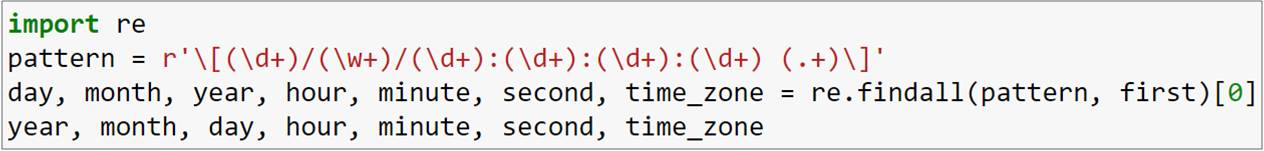
\includegraphics[scale=.6]{Bild25}
    	\end{figure}
    	You will also see code that uses re.search instead of re.findall.
    	\begin{itemize}
    	    \item Beyond the scope of our lecture today.
    	\end{itemize}
    	\begin{figure}
    	    \centering
    	    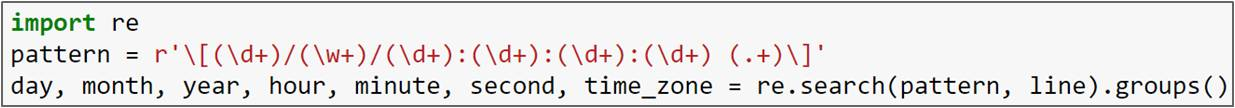
\includegraphics[scale=.65]{Bild26}
    	\end{figure}
	\end{frame}
\end{document}